%% History:

% One-page layout: (proof-)reading on display
%%%% \documentclass[11pt,oneside,a4paper]{book}
% Two-page layout: final printing
\documentclass[11pt,twoside,a4paper]{book}   
%=-=-=-=-=-=-=-=-=-=-=-=--=%
% The user of this template may find useful to have an alternative to these 
% officially suggested packages:
\usepackage[czech, english]{babel}
\usepackage[T1]{fontenc} % pouzije EC fonty 
% pripadne pisete-li cesky, pak lze zkusit take:
% \usepackage[OT1]{fontenc} 
\usepackage[utf8]{inputenc}
\usepackage{lscape}
\usepackage{amsmath,amssymb,latexsym}
\usepackage{epstopdf} %converting to PDF

%\usepackage{float}
\usepackage{floatflt}


%=-=-=-=-=-=-=-=-=-=-=-=--=%
% In case of problems with PDF fonts, one may try to uncomment this line:
%\usepackage{lmodern}
%=-=-=-=-=-=-=-=-=-=-=-=--=%
%=-=-=-=-=-=-=-=-=-=-=-=--=%
% Depending on your particular TeX distribution and version of conversion tools 
% (dvips/dvipdf/ps2pdf), some (advanced | desperate) users may prefer to use 
% different settings.
% Please uncomment the following style and use your CSLaTeX (cslatex/pdfcslatex) 
% to process your work. Note however, this file is in UTF-8 and a conversion to 
% your native encoding may be required. Some settings below depend on babel 
% macros and should also be modified. See \selectlanguage \iflanguage.
%\usepackage{czech}  %%%%%\usepackage[T1]{czech} %%%%[IL2] [T1] [OT1]
%=-=-=-=-=-=-=-=-=-=-=-=--=%

%%%%%%%%%%%%%%%%%%%%%%%%%%%%%%%%%%%%%%%
% Styles required in your work follow %
%%%%%%%%%%%%%%%%%%%%%%%%%%%%%%%%%%%%%%%
\usepackage{graphicx}
%\usepackage{indentfirst} %1. odstavec jako v cestine.

\usepackage{k336_thesis_macros} % specialni makra pro formatovani DP a BP
 % muzete si vytvorit i sva vlastni v souboru k336_thesis_macros.sty
 % najdete  radu jednoduchych definic, ktere zde ani nejsou pouzity
 % napriklad: 
 % \newcommand{\bfig}{\begin{figure}\begin{center}}
 % \newcommand{\efig}{\end{center}\end{figure}}
 % umoznuje pouzit prikaz \bfig namisto \begin{figure}\begin{center} atd.


%%%%%%%%%%%%%%%%%%%%%%%%%%%%%%%%%%%%%
% Zvolte jednu z moznosti 
% Choose one of the following options
%%%%%%%%%%%%%%%%%%%%%%%%%%%%%%%%%%%%%
% \newcommand\TypeOfWork{Diplomová práce} \typeout{Diplomova prace}
 \newcommand\TypeOfWork{Master's Thesis}   \typeout{Master's Thesis} 
% \newcommand\TypeOfWork{Bakalářská práce}  \typeout{Bakalarska prace}
% \newcommand\TypeOfWork{Bachelor's Project}  \typeout{Bachelor's Project}


%%%%%%%%%%%%%%%%%%%%%%%%%%%%%%%%%%%%%
% Zvolte jednu z moznosti 
% Choose one of the following options
%%%%%%%%%%%%%%%%%%%%%%%%%%%%%%%%%%%%%
% nabidky jsou z: http://www.fel.cvut.cz/cz/education/bk/prehled.html

%\newcommand\StudProgram{Elektrotechnika a informatika, dobíhající, Bakalářský}
%\newcommand\StudProgram{Elektrotechnika a informatika, dobíhající, Magisterský}
% \newcommand\StudProgram{Elektrotechnika a informatika, strukturovaný, Bakalářský}
 \newcommand\StudProgram{Open Informatics}
% \newcommand\StudProgram{Softwarové technologie a management, Bakalářský}
% English study:
% \newcommand\StudProgram{Electrical Engineering and Information Technology}  % bachelor programe
% \newcommand\StudProgram{Electrical Engineering and Information Technology}  %master program


%%%%%%%%%%%%%%%%%%%%%%%%%%%%%%%%%%%%%
% Zvolte jednu z moznosti 
% Choose one of the following options
%%%%%%%%%%%%%%%%%%%%%%%%%%%%%%%%%%%%%
% nabidky jsou z: http://www.fel.cvut.cz/cz/education/bk/prehled.html

%\newcommand\StudBranch{Výpočetní technika}   % pro program EaI bak. (dobihajici i strukt.)
\newcommand\StudBranch{Artificial Intelligence}   % pro prgoram EaI mag. (dobihajici i strukt.)
%\newcommand\StudBranch{Softwarové inženýrství}            %pro STM
%\newcommand\StudBranch{Web a multimedia}                  % pro STM
%\newcommand\StudBranch{Computer Engineering}              % bachelor programe
%\newcommand\StudBranch{Computer Science and Engineering}  % master programe

\newcounter{Definition}

%%%%%%%%%%%%%%%%%%%%%%%%%%%%%%%%%%%%%%%%%%%%
% Vyplnte nazev prace, autora a vedouciho
% Set up Work Title, Author and Supervisor
%%%%%%%%%%%%%%%%%%%%%%%%%%%%%%%%%%%%%%%%%%%%

\newcommand\WorkTitle{Protein function prediction from protein structure using machine learning}
\newcommand\FirstandFamilyName{Bc. Jáchym Barvínek}
\newcommand\Supervisor{doc. Ing. Filip Železný, Ph.D.}


% Pouzijete-li pdflatex, tak je prijemne, kdyz bude mit vase prace
% funkcni odkazy i v pdf formatu
\usepackage[
pdftitle={\WorkTitle},
pdfauthor={\FirstandFamilyName},
bookmarks=true,
colorlinks=true,
breaklinks=true,
urlcolor=red,
citecolor=black,
linkcolor=black,
unicode=true,
]
{hyperref}




\begin{document}

%%%%%%%%%%%%%%%%%%%%%%%%%%%%%%%%%%%%%
% Zvolte jednu z moznosti 
% Choose one of the following options
%%%%%%%%%%%%%%%%%%%%%%%%%%%%%%%%%%%%%
%\selectlanguage{czech}
\selectlanguage{english} 

% prikaz \typeout vypise vyse uvedena nastaveni v prikazovem okne
% pro pohodlne ladeni prace


\iflanguage{czech}{
	 \typeout{************************************************}
	 \typeout{Zvoleny jazyk: cestina}
	 \typeout{Typ prace: \TypeOfWork}
	 \typeout{Studijni program: \StudProgram}
	 \typeout{Obor: \StudBranch}
	 \typeout{Jmeno: \FirstandFamilyName}
	 \typeout{Nazev prace: \WorkTitle}
	 \typeout{Vedouci prace: \Supervisor}
	 \typeout{***************************************************}
	 \newcommand\Department{Katedra počítačů}
	 \newcommand\Faculty{Fakulta elektrotechnická}
	 \newcommand\University{České vysoké učení technické v Praze}
	 \newcommand\labelSupervisor{Vedoucí práce}
	 \newcommand\labelStudProgram{Studijní program}
	 \newcommand\labelStudBranch{Obor}
}{
	 \typeout{************************************************}
	 \typeout{Language: english}
	 \typeout{Type of Work: \TypeOfWork}
	 \typeout{Study Program: \StudProgram}
	 \typeout{Study Branch: \StudBranch}
	 \typeout{Author: \FirstandFamilyName}
	 \typeout{Title: \WorkTitle}
	 \typeout{Supervisor: \Supervisor}
	 \typeout{***************************************************}
	 \newcommand\Department{Department of Computer Science and Engineering}
	 \newcommand\Faculty{Faculty of Electrical Engineering}
	 \newcommand\University{Czech Technical University in Prague}
	 \newcommand\labelSupervisor{Supervisor}
	 \newcommand\labelStudProgram{Study Programme} 
	 \newcommand\labelStudBranch{Field of Study}
}




%%%%%%%%%%%%%%%%%%%%%%%%%%    Poznamky ke kompletaci prace
% Nasledujici pasaz uzavrenou v {} ve sve praci samozrejme 
% zakomentujte nebo odstrante. 
% Ve vysledne svazane praci bude nahrazena skutecnym 
% oficialnim zadanim vasi prace.
{
\pagenumbering{roman} \cleardoublepage \thispagestyle{empty}
\chapter*{Na tomto místě bude oficiální zadání vaší práce}
\begin{itemize}
\item Toto zadání je podepsané děkanem a vedoucím katedry,
\item musíte si ho vyzvednout na studiijním oddělení Katedry počítačů na Karlově náměstí,
\item v jedné odevzdané práci bude originál tohoto zadání (originál zůstává po obhajobě na katedře),
\item ve druhé bude na stejném místě neověřená kopie tohoto dokumentu (tato se vám vrátí po obhajobě).
\end{itemize}
%\newpage
}

%%%%%%%%%%%%%%%%%%%%%%%%%%    Titulni stranka / Title page 

\coverpagestarts

%%%%%%%%%%%%%%%%%%%%%%%%%%%    Podekovani / Acknowledgements 

\acknowledgements
\noindent
%Access to computing and storage facilities owned by parties and projects contributing to the National Grid Infrastructure MetaCentrum, provided under the programme "Projects of Large Infrastructure for Research, Development, and Innovations" (LM2010005), is greatly appreciated.
%Access to the CERIT-SC computing and storage facilities provided under the programme Center CERIT Scientific Cloud, part of the Operational Program Research and Development for Innovations, reg. no. CZ. 1.05/3.2.00/08.0144, is greatly appreciated.
Computational resources were provided by the MetaCentrum under the program LM2010005 and the CERIT-SC under the program Centre CERIT Scientific Cloud, part of the Operational Program Research and Development for Innovations, Reg. no. CZ.1.05/3.2.00/08.0144.



%%%%%%%%%%%%%%%%%%%%%%%%%%%   Prohlaseni / Declaration 

\declaration{In Prague}
%\declaration{In Kořenovice nad Bečvárkou on May 15, 2008}


%%%%%%%%%%%%%%%%%%%%%%%%%%%%    Abstract 
 
\abstractpage

Translation of Czech abstract into English.

% Prace v cestine musi krome abstraktu v anglictine obsahovat i
% abstrakt v cestine.
\vglue60mm

\noindent{\Huge \textbf{Abstrakt}}
\vskip 2.75\baselineskip

\noindent
Abstrakt práce by měl velmi stručně vystihovat její podstatu. Tedy čím se práce zabývá a co je jejím výsledkem/přínosem.

\noindent
Očekávají se cca 1 -- 2 odstavce, maximálně půl stránky.

%%%%%%%%%%%%%%%%%%%%%%%%%%%%%%%%  Obsah / Table of Contents 

\tableofcontents


%%%%%%%%%%%%%%%%%%%%%%%%%%%%%%%  Seznam obrazku / List of Figures 

\listoffigures


%%%%%%%%%%%%%%%%%%%%%%%%%%%%%%%  Seznam tabulek / List of Tables

\listoftables


%**************************************************************

\mainbodystarts
% horizontalní mezera mezi dvema odstavci
%\parskip=5pt
%11.12.2008 parskip + tolerance
\normalfont
\parskip=0.2\baselineskip plus 0.2\baselineskip minus 0.1\baselineskip

% Odsazeni prvniho radku odstavce resi class book (neaplikuje se na prvni 
% odstavce kapitol, sekci, podsekci atd.) Viz usepackage{indentfirst}.
% Chcete-li selektivne zamezit odsazeni 1. radku nektereho odstavce,
% pouzijte prikaz \noindent.

%**************************************************************

% Pro snadnejsi praci s vetsimi texty je rozumne tyto rozdelit
% do samostatnych souboru nejlepe dle kapitol a tyto potom vkladat
% pomoci prikazu \include{jmeno_souboru.tex} nebo \include{jmeno_souboru}.
% Napr.:
% \include{1_uvod}
% \include{2_teorie}
% atd...

%*****************************************************************************
\chapter{Introduction}
Identification of protein functions is a key task in medicinal and biological research.
It is currently mostly done by laboratory experimental methods.
Laboratory processes could be costly and time-consuming. 
Being able to automate this process computationally would therefore save resources
and made the research easier.
Even approximate solutions are useful as the can give researchers guidance where
to start with protein function identification.

Automated protein function prediction is then one of the classical problems in bioinformatics. 
This problem is complicated and computationally challenging and all existing solutions
are only approximate and based on strongly simplifying assumptions.
It is still an active area of research various approaches are being explored. 
In this work we focus on methods of relational machine learning (elaborated on in \cite{kuzelka}\cite{relf})
that ware applied to to prediction of DNA-binding protein function in \cite{szabova}.

A major advantage of relational learning approach is that it generates protein's local structural patterns
(likely to determine protein's function) which can be interpreted and examined chemically.

This work assumes that reader knows
the techniques of well-know machine learning algorithms (mainly Suppor Vector Machines),
Bayesian networks
and the formalism of first order logic and graph theory.

\section{Problem statement}

This work examines the application of techniques used in \cite{szabova} towards a more ambitious goal:
Prediction of arbitrary protein function
defined by the Gene Ontology (GO) \cite{go}\cite{gores},
provided that there is enough training data for each particular function that we'd like to be able predict.

The basic workflow is the following:
First, a non-redundant data set of proteins is extracted from Protein Data Bank \cite{pdb}.
The data set non-redundancy is achieved using technique described in \cite{maxind}.
The information about each protein in converted to a relational form, 
which in our case is a conjunction of positive, ground, first-order logic literals.
The algorithm RelF \cite{relf} is then used to find characteristic features
for a given protein function.
Similarly to the work \cite{szabova}, the learned relational features are further
processed by the classical machine learning algorithm Support Vector Machines
to predict if a protein has a single given function.
Subsequently a technique developed in \cite{bnet} based on Bayesian networks is applied to make the classification
results consistent with the Gene Ontology,
i.e. that if a protein is predicted to have a certain function
(identified by a GO term in the \emph{molecular function} namespace),
then all functions defined by all more general GO terms should also be predicted.

Finally, an evaluation of performance of this approach to protein function classification is done. 

%Úvod charakterizující kontext zadání, případně motivace.
%\cite{kuzelka} \cite{szabova} \cite{bnet} \cite{relf} \cite{sklearn} \cite{go} \cite{gores} \cite{maxind}

\section{Thesis overview}
TODO

%Výsledná struktura vaší práce a názvy a rozsahy jednotlivých kapitol
%se samozřejmě budou lišit podle typu práce a podle konkrétní povahy zpracovávaného tématu.
%Níže uvedená struktura práce odpovídá \textit{práci implementační}, viz \cite{infodp} respektive \cite{infobp}. 


\chapter{Biomolecular background}
In this chapter, some basic facts about proteins
necessary for understanding this work are presented.

Proteins are macromolecules composed of one or more chains of amino acid residues
connected by peptide bond.
Proteins have broad spectrum of functions in living organisms, including for example 
various types of catalytic activity, signal transmission or DNA manipulation.

In organisms proteins are encoded by genes. 
For the close correspondence between genes and proteins,
the terms ``gene'' and ``protein'' are interchangeable for the purpose of this thesis
(especially in the context of Gene Ontology, which we actually use more like ``protein function ontology''.)

%These amino acids are chained by peptide bond.
\paragraph{Protein structural levels} With rare exceptions, that we won't consider, each of the amino acids is one the
so-called proteinogenic amino acids (see table \ref{tab:aaprops}). 
This chain as a linear sequence of symbols is defined to be the protein's \emph{primary structure}.
There are also several types of structures that appear in proteins locally and are common among
proteins of various types.
They could be though of as a higher-level structural units. This is known as the \emph{secondary structure}
of a protein. In this work, the following types of secondary structure are distinguished:
\begin{itemize}
 \item $\alpha$-helix
 \item $\beta$-bridge
 \item $\beta$-sheet
 \item $3_{10}$ helix
 \item $\pi$-helix
 \item Turn (hydrogen bonded)
 \item Bend
 \item Unknown
\end{itemize}
The protein's geometric shape in three dimensional space is called the \emph{tertiary structure}. 
Finally, multiple tertiary structures (strands) can unite into \emph{quaternary structure}.
In this work, only primary, secondary and tertiary structures are considered for computations.
Proteins that exhibit quaternary structure are present in data, but are dealt with per-strand; 
the quaternary structure itself is ignored.

Interacting with other molecules (including the composition of a quaternary structure)
may temporarily or even permanently change the protein's lower level structures,
especially tertiary structure.
A change in protein's spatial confomation may also change the set of functions
it exhibits. 
In other ways, changing of structure can be part of the protein's function:
For example a protein with DNA-binding function will somewhat change it's tertiary
structure when bound to a DNA molecule, but it doesn't mean that it lacks this
function when unbound.

\begin{landscape}
\begin{figure}[h]
\begin{center}
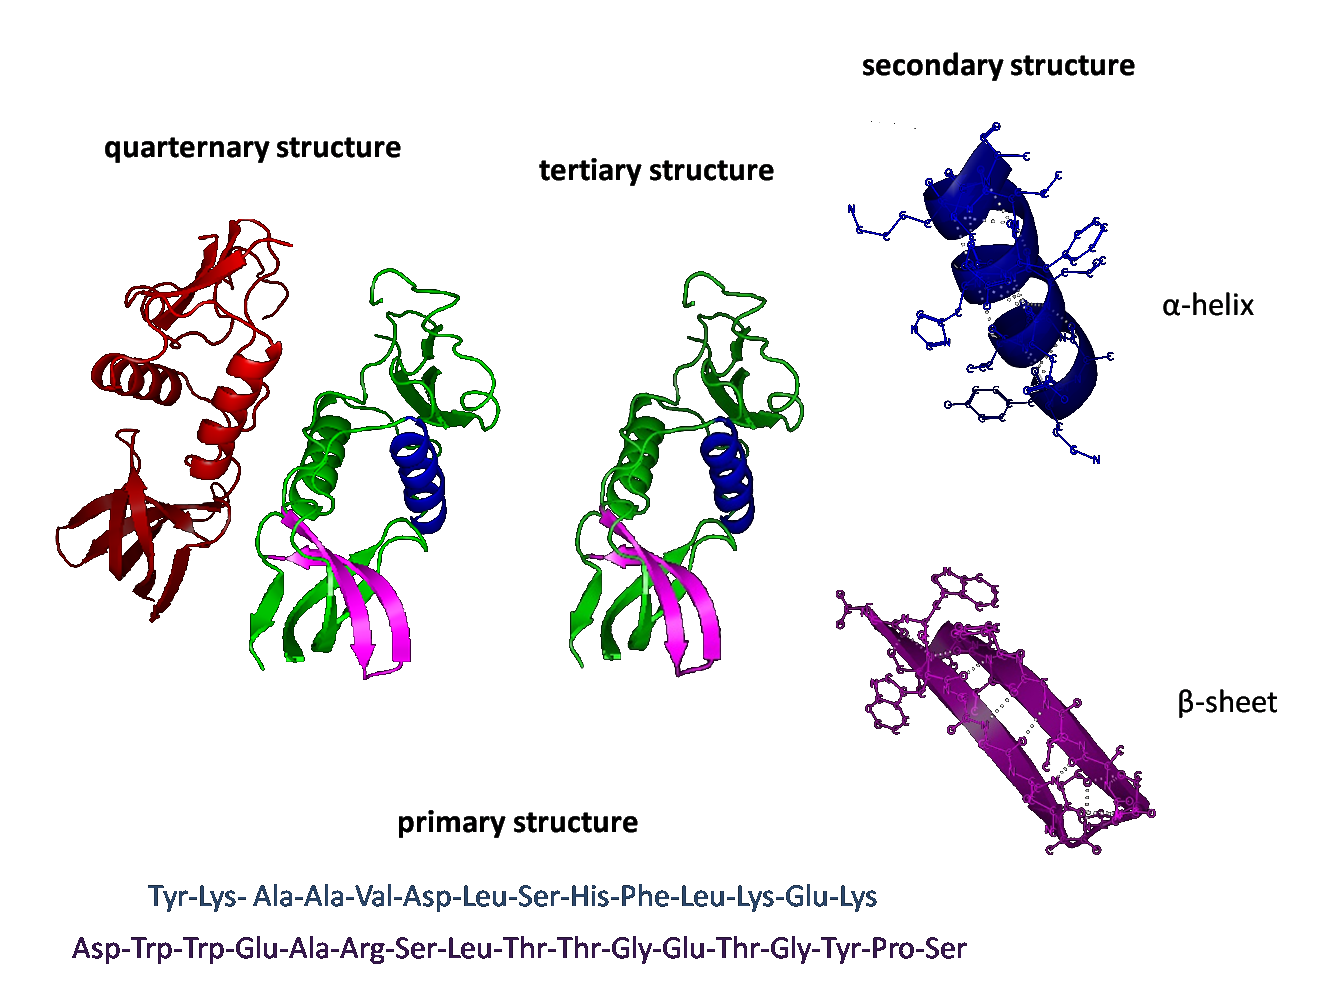
\includegraphics[width=21cm]{figures/Protein_structure}
\caption[Structure levels of the protein 1EFN]{Structure levels of the protein 1EFN. Adapted from \emph{Wikipedia}}
\label{fig:Protein_structure}
\end{center}
\end{figure}
\end{landscape}


%*****************************************************************************
%\begin{itemize}
%\item Popis řešeného problému, vymezení cílů DP/BP a požadavků na implementovaný systém.
%\item Popis struktury DP/BP ve vztahu k vytyčeným cílům.
%\item Rešeršní zpracování existujících implementací, pokud jsou známy.
%\end{itemize}

%*****************************************************************************
\chapter{Solution design}
% Analýza a návrh implementace (včetně diskuse různých alternativ a volby implementačního prostředí).

\section{Data sources and preprocessing}
\label{sec:data}
In this section, the nature and sources of the input data used later for machine learning are described.

\subsection{Gene Ontology}
\label{ssec:go}
Gene Ontology (GO) \cite{go} is a representation of relationships among various \emph{terms} identifying common (species-independent)
biological processes, cellular components and molecular functions.
The GO terms definitions and relationships among them are provided by human experts. 
In this work, we're only interested in terms identifying molecular functions and the $\prec$ generality relation among them
(denoted here by the symbol $\prec$).
These terms together with the $\prec$ relation form a directed acyclic graph, with a single leaf (node with zero outgoing edges),
which represents the
most general (i.e. arbitrary) molecular function. 
The GO terms themselves are unambiguously identified either by a numerical id (e.g. GO:0046872) or a human-readable name
(``metal ion binding'', in this case).
The $\prec$ relationship maps a term to more general ones. So for example GO:0046872 $\prec$ GO:0043169 (``cation binding'')
 and GO:0043169  $\prec$ GO:0043167 (``ion binding'').
 The $\prec$ relation is implicitly transitive,
 thus for for example also ``metal ion binding''  $\prec$ ``ion binding''.
 
The ontology used in this thesis is the \texttt{go-basic.obo} \cite{gores} \url{http://geneontology.org/page/download-ontology} provided by the Gene Ontology Consortium. 
It serves two purposes in this work:
1) In the initial steps of the work, it is a simple list of protein functions.
The molecular function terms are the protein functions studied in this work.
In this context, general functions are studied alongside specific ones. 
2) The underlying directed acyclic graph is used as the skeleton for construction of the 
Bayesian network in the consistency correction step. 

There are over 10000 terms in the ``molecular function'' namespace of Gene Ontology.
A certain subset has to be selected because of two reasons:
1) Most terms are too specific and have very few (of none at all) proteins associated with them
and therefore are useless for machine learning.
2) The performed computations are difficult and computational resources are finite.
Therefore only the terms which have the most proteins associated with them are used.
Due to the transitivity of the $\prec$ relation,
these also happen to be some of the most general terms in the ontology.                                                                                                                                                                                                                                                                                                                                                                                                                                                                                                                                                                                                                                                                                                                                                                                                                                                                                                                                                                                         
                                                                                                                                                                                                                                                                                                                                                                                                                                                                                                                                                                                                                                                                                                                                               

\subsection{Proteins}
\label{ssec:proteins}
Data about proteins used in this work were extracted from Research Collaboratory for Structural Bioinformatics (RCSB) Protein Data Bank (PDB) \cite{pdb}.
PDB currently publishes over 100000 entries containing information about identified existing protein structures.
The entries contain various details about the molecular structure,
but only the protein identifier and structure are used in this work.
The following data are thus extracted from each used entry:
\begin{itemize}
 \item Protein name -- identifier. If a protein has a quaternary structure,
 it is separated into polypeptide strands each of which has a unique identifier and associated GO terms
 (possibly distinct among strands of the same complex.)
 \item Primary structure -- the linear chain of amino acids.
 Many proteins in PDB have unidentified terminating (or sometimes other) amino acid residues.
 Only proteins with more than 90\% of it's primary structure identified are used.
 The relational representation of proteins offers a natural way of dealing with missing amino
 acid residue information as we will see later.
 \item Secondary structure -- the information describing to which type of secondary structure each amino acid residue belongs.
 It could be of unknown/unidentified type. In an average PDB protein entry containing secondary structure information, 76\% of residues have an associated secondary structure.
 Only proteins with at least some information about secondary structure are used.
 \item Tertiary structure -- PDB contains detailed data about positions of various atoms in each amino acid residue.
 This information cannot be used in completeness for tractability reasons. 
 Only the coordinates of the $\alpha$-carbon on each amino acid residue are used in computations.
 Before the relational learning phase, coordinates are used to calculate distances between $\alpha$-carbons discretized to 2Å.
 Note, however, that PDB entries often have resolution worse than 2Å.
 This is a potential problem in the data.
 The rationale behind including entries with worse resolution is that the data set will be large and thus the solution
 is expected to be robust towards position measurement errors.
\end{itemize}

Another information that PDB provides and could be used in learning is the ligand information.
(\emph{Ligand} is the active site of the protein, for example a binding site.) 
The idea is that protein function is mostly determined by the ligand and the structural parts 
distant from the ligand are not so important.
If only information about residues with certain distance from ligands were used,
the data set size could be greatly reduced possibly bearing almost the same information
exploitable for learning.
Hence, it would be feasible to learn from larger data set and train a better classifier.
Application of this idea was rejected in this work,
because it is unclear how much is ligand information defining for each GO term,
but it is reasonable to assume that it varies. 
Therefore the evaluation results would be biased and performance of prediction
on different GO terms could not be compared.
It is, however, an interesting problem for future research in this field.

\paragraph{Data location} Local mirrors of PDB databases were used in this work (see \url{http://www.rcsb.org/pdb/static.do?p=download/ftp/index.html}.)
Secondary structures in FASTA format are available from \url{http://www.rcsb.org/pdb/static.do?p=download/http/index.html}.)
Protein annotations, i.e. data that associate GO terms with actual genes (proteins -- PDB entries), were downloaded from
\url{http://geneontology.org/page/download-annotations}, 
the file \url{http://geneontology.org/gene-associations/gene_association.goa_pdb.gz}.
Proteins, that are not associated with any of the studied functions are discarded from the data set.

\paragraph{Species} The association file also contain information about the biological taxon from which the protein was taken.
In this work only proteins from \emph{Homo sapiens} were used.
(UniProt taxon id 9609 identifies \emph{Homo sapiens} in the association file.) 
The assumption behind this is that learning on a single organism should result in
greater prediction precision for that organism.
With relational learning methods however, it would be interesting to study, if there exist protein
structural patterns for a given function, that are common even in evolutionary distant species.

\paragraph{Protein confomations} In the work \cite{szabova} where similar methods were used to predict DNA-binding protein 
function, only proteins in either their bound or unbound confomation were used.
Arranging the data set to include only proteins of specific type of
confomation makes sense if: 1) It is easy to determine this confomation type 
before presenting a yet unidentified protein to the classifier. 
2) This specific confomation is defined for the studied function.
For binding proteins, this confomation type is either the bound
or unbound confomation.
In this work, the confomation is not taken into account, though.
First, it is not obvious how to define the right confomation
type for each function, since also non-binding functions
are studied here (for example catalytic activity).
Although binding proteins form a large subset of all the proteins
in the dataset, using only (un)bound confomations  for them  would introduce
some bias in the comparison of classification results.
An advantage of not using specific confomation is that 
the classifier should then learn to recognize 
the protein in any confomation.
(Albeit possibly with lesser precision.) 

\subsection{Non-redundant data set}
\label{ssec:redundancy}
One problem with Protein Data Bank is that it contains many redundant entries --
proteins that are almost identical.
That can be caused for example by a minor mutation that preserves the protein's function.
Redundant entries should be removed from the data being used for machine learning for two reasons:
1) They bloat the data set making the learning more computationally difficult.
2) As a consequence of redundancy, many similar entries could appear in both training and testing data set
which would yield overly optimistic results when evaluated, 
while the classifier could actually be overfitted.
It is not obvious, how redundancy or protein similarity should exactly be defined,
but in this work the approach to redundancy and it's removal described by \cite{maxind} is loosely followed.

The basic idea is the following: 
Assume, that there exists a reasonable similarity relation on the protein data set. 
This relation is represented by a graph -- distinct proteins are nodes and there
is a edge between each two proteins that are similar by the given relation.
We define a non-redundant data set a set of proteins such that no two are similar.
In other words, we would like to find a set of nodes in that graph such that no two are adjacent
and we prefer this set to be the largest possible.
This is a non-formal definition of the maximum independent set problem in graph theory.
It is known to be NP-HARD, but fortunately a heuristic solution suffices.
The following simple heuristic is employed:
Start with empty independent set.
Until no more nodes can be added to the independent set,
iteratively pick a random node from the graph,
put it to the independent set and remove all adjacent nodes from the graph.
Repeat the whole process several times and select the best solution (largest independent set).

Now, the similarity of two proteins is defined as the inverse of their local alignment \emph{E value} computed by BLAST \cite{blast} \cite{blastp}.
BLAST is an algorithm that finds and measures local alignment of two sequences,
in our case of the sequences of amino acid residues of two proteins. 
This means, it is a distance measure based purely on the primary structure of proteins.
Let us denote by $S = BLAST(A,B)$ the score of alignment (BLOSUM62 substitution matrix is used) 
of two proteins $A, B$.
The BLAST program then also computes a number called \emph{Expect value} or simply \emph{E value}, 
defined as follows:
\[ E = K \cdot l_A \cdot l_B \cdot e^{-\lambda \cdot S}, \]
where $l_A$ and $l_B$ are lengths of the sequences $A,B$ respectively and $K$ and $\lambda$ are constant parameters.
The E value can be interpreted as the expected number of proteins present in a database of a given size
that would match witch score $S$ or higher simply by chance.
Here, the E value is used in the following way: We define that $A$ is similar to $B$ if $E < T$ for some threshold $T$.
Note, that generally $BLAST(A,B) \neq BLAST(B,A)$,
so the closure under symmetry for the similarity relation is actually used.
The question remains, how to choose the value $T$.
For the purpose of this work $T = 10^{-50}$ was used.
This choice was made intuitively and ad-hoc (to keep the data set large enough, see below),
since the author is not aware of any theory that would guide such decision.
But at least to illustrate what the value means, here is an example of best local alignment match
for two variants of the lysozyme protein (PDB ids 132L and 1QSW), for which the \texttt{blastp} program computed E value of $10^{-50}$
(i.e. no proteins that would be ``more similar'' appear in the data set together.):
\begin{minipage}{\linewidth}
\begin{verbatim}


132L: KVFGRCELAAAMKRHGLDNYRGYSLGNWVCAAKFESNFNTQATNRNT-DGSTDYGILQINSRWWCNDGRTP
Match KVF RCELA  +KR G+D YRG SL NW+C AK+ES +NT+ATN N  D STDYGI QINSR+  NDG+TP
1QSW: KVFERCELARTLKRLGMDGYRGISLANWMCLAKWESGYNTRATNYNAGDRSTDYGIFQINSRYCANDGKTP
      GSRNLCNIPCSALLSSDITASVNCAKKIVSDGNGMNAWVAWRNRCKGTDVQAWIRGCRL
      G+ N C++ CSALL  +I  +V CAK++V D  G+ AWVAWRNRC+  DV+ +++GC
      GAVNACHLSCSALLQDNIADAVACAKRVVRDPQGIRAWVAWRNRCQNRDVRQYVQGCGV
      
      
\end{verbatim}
\end{minipage}
Here, amino-acid residues are encoded by the standard single-letter code (see table \ref{tab:aaprops} for reference). 

Some disadvantages follow from using BLAST as distance function.
There could be some proteins which have the same primary structure, 
but can exist in varying spatial confomation exhibiting different functions.
It would do no harm to include both in the data set if the difference is large enough.
For BLAST, however, they will be indistinguishable and as a result 
only one of them will appear in the final dataset.

\section{Relational learning}
In this section, approach to machine learning using relational learning based on structural patterns
is briefly explained and 
it's application to the protein function prediction in this work is explained.

\subsection{Relational representation of proteins}
\label{ssec:relrepr}
Let us first define how proteins can be represented as first order logic propositions.
The data will be fed to the RelF algorithm,
which expects a set of conjunctions of positive ground literals.
The representation should therefore respect this limitation.

Relational representation of data is naturally discrete.
The basic discrete unit of protein is a single amino acid residue,
so our relational description of a protein consists mainly
of literals describing that there is a certain relationship between 
two residues or that a residue has a certain property.
(In theory, it could be more than two, but that is not used here.)
Further, discretized information about polarity and electrical charge
is encoded in the rest of each conjunction as \emph{background knowledge}.

Let us start with a simple step-by-step example illustrating how information about
peptide primary structure could be encoded.
Assume for example a peptide Glu-Pro-Asp, a subsequence of the protein 1APJ.
First, let us encode the simple fact,
that there are three distinct residues, as the following conjunction:
\[ Res(r1) \land Res(r2) \land Res(r3). \]
Now we can add the information about the residue type. The conjunction becomes:
\[ Res(r1) \land Type(r1, glu) \land Res(r2) \land Type(r2, pro) \land Res(r3) \land Type(r3, asp). \]
The predicate $Res$ may seem redundant now.
The reason why it is included is that it makes it algorithmically easier to deal with incomplete information about a residue.
It is exploited in templates for the RelF algorithm later.
This still contains no information about the primary structure, 
which could be inserted in the following way:
\begin{align*}
Res(r1)& \land Type(r1, glu) \land \\
Res(r2)& \land Type(r2, pro) \land Next(r1, r2) \land \\
Res(r3)& \land Type(r3, asp) \land Next(r2, r3). 
\end{align*}
we may not know the residue type, but perhaps we know some other information about it
(for example the $Next$ relation)


The following information is actually encoded in the implementation of this work:
\begin{itemize}
 \item Residue type -- simply the type of each amino acid, if it is known.
 \item Distance between residues -- distances of $\alpha$-carbons discretized to 2Å with upper bound 14Å.
 This is a tertiary structure infromation, but it also implicitly includes primary structure 
 as neighboring amino acid residues are not too distant.
 \item Secondary structure type of which the residue is part.
 \item Background information -- polarity (polar / nonpolar) and electrical charge (positive / neutral / negative)
 information about amino acids.
 No information about amino acids outside this background knowledge is used.
\end{itemize}

The Glu-Pro-Asp subsequence of 1APJ from the example is then encoded in the following way:
\begin{align*}
&Res(r1) \land Type(r1, glu) \land SecStr(r1, turn) \land \\
&Res(r2) \land Type(r2, pro) \land SecStr(r2, turn) \land Dist(r1, r2, 8) \\
&Res(r3) \land Type(r3, asp) \land SecStr(r3, bend) \land Dist(r2, r3, 8) \\
&Polarity(glu, polar) \land Charge(glu, negative) \land \\
&Polarity(pro, nonpolar) \land Charge(pro, neutral) \land \\
&Polarity(asp, polar) \land Charge(asp, negative).
\end{align*}

Note, that we can also think of the conjunction as a certain first order logic interpretation:
it defines for which constants the used predicates are true.
Each protein in the data set is converted to this relational form.
It is obvious that this representation of proteins is great simplification.
The hope is that this model captures some of the essential properties of the 
protein while it is computationally feasible to work with such model.

Also note, how easy it is in this relational representation to deal with missing data:
If for example we do not know the secondary structure in which a certain amino acid 
residue occurs or the polarity of an amino acid in case of Asx and Glx (see Table \ref{tab:aaprops})
or even if there is completely missing information about an amino acid residue,
we can simply omit the literals relevant to this information.
So for example if we did not know the secondary structure of $r1$,
we would drop the literal $SecStr(r1, turn)$ in the above example.
However, this is not completely correct approach and it introduces noise in the data:
The algorithms that later work with this data cannot distinguish information
that is not known and information that is know to be false.
For example,
not including $SecStr(r1, turn)$ because we do not know it although it is true
is very different from not including $Type(r1, ala)$ which is know to be false,
yet these two cases are represented the same way.

\begin{table}
\begin{center}
 \begin{tabular}{lccrr}
\textbf{Name} & \textbf{Code} & \textbf{Abbreviation} & \textbf{Charge} & \textbf{Polarity} \\
\hline
Alanine & A & Ala & neutral & nonpolar  \\ \hline
Arginine & R & Arg & positive & polar  \\ \hline
Asparagine & N & Asn & neutral & polar \\ \hline 
Aspartic acid & D & Asp & negative & polar  \\ \hline
Asparagine or aspartic acid & B & Asx & ? & polar \\ \hline 
Cysteine & C & Cys & neutral & nonpolar  \\ \hline
Glutamine & Q & Gln & neutral & polar  \\ \hline
Glutamic acid & E & Glu & negative & polar \\ \hline
Glutamic acid or glutamine & Z & Glx & ? & polar \\ \hline
Glycine & G & Gly & neutral & nonpolar \\ \hline
Histidine & H & His & neutral & polar \\ \hline
Isoleucine & I & Ile & neutral & nonpolar \\ \hline
Leucine & L & Leu & neutral & nonpolar \\ \hline
Lysine & K & Lys & positive & polar \\ \hline
Methionine & M & Met & neutral & nonpolar  \\ \hline
Phenylalanine & F & Phe & neutral & nonpolar  \\ \hline
Proline & P & Pro & neutral & nonpolar \\ \hline
Pyrrolysine & O & Pyl  & neutral & polar  \\ \hline
Selenocysteine & U & Sec & negative & polar  \\ \hline
Serine & S & Ser & neutral & polar  \\ \hline
Threonine & T & Thr & neutral & polar \\ \hline
Tryptophan & W & Trp & neutral & nonpolar   \\ \hline
Tyrosine & Y & Tyr & neutral & polar  \\ \hline
Valine & V & Val & neutral & nonpolar \\ \hline
Leucine or islueucine & J & Xle & neutral & nonpolar \\ \hline
Unknown or unidentified & X & Xxx & ? & ? \\ \hline
\end{tabular}
\caption{Proteinogenic amino acids and their used properties}
\label{tab:aaprops}
\end{center}
\end{table}

\subsection{Learning with relational features}
A technique called \emph{propositionalization} is employed in this work. 
Generally, propositionalization is the transformation of a relational data set
into an attribute-value data set.
Attribute-value data set can then be used as input to many
state of the art machine learning algorithms, such as 
Support Vector Machines.
In this work, we use the RelF algorithm to perform the propositionalization,
but in principle different supervised propositionalization
techniques could be examined in this context.
The TreeLiker software (\url{http://ida.felk.cvut.cz/treeliker/TreeLiker.html})
was used as the implementation of RelF here.

A brief description of the propositionalization idea used in RelF algorithm follows.
For more detailed description, see the article \cite{relf}.
RelF could be classified as an inductive logic programming (ILP) algorithm.
There are two important notions (\emph{$\theta$-subsumption} and \emph{$\theta$-reduction})
in many ILP problems including the RelF propositionalization technique.
Further, the notion of \emph{tree-like} conjunction property is needed 
for understanding of the propositionalization results.
So let us first remind their definitions (adapted from \cite{szabova},\cite{relf}): 

\paragraph{Definition} ($\theta$-subsumption) Let $A,B$ be clauses. 
The clause $A$ \emph{$\theta$-subsumes} $B$ (written $A \preceq_{\theta} B$)
iff there exists a substitution $\theta$ such that $ A \theta \subseteq B$.
If $A \preceq_{\theta} B$ and $B \preceq_{\theta} A$, we call $A$ and $B$ 
$\theta$-equivalent (written $A \approx_{\theta} B$).

\paragraph{ } The motivation for the definition of $\theta$-subsumption is that it is a decidable
(but incomplete) approximation of the covering (semantic consequence, $\vDash$) relation,
which itself is undecidable in general.
To be precise, if $A \preceq_{\theta} B$ then $A \vDash B$. \cite{plotkin}

\paragraph{Definition} ($\theta$-reduction) Let $A$ be a clause.
If there exists a $R$, such that $|R| < |A|$ and $A \approx_{\theta} R$,
we say that $A$ is \emph{$\theta$-reducible}. 
A minimal such $R$ is called the \emph{$\theta$-reduction} of $A$.

\paragraph{Definition}   (Tree-like conjunction) A first-order logic conjunction (hypergraph) $C$
is said to be \emph{tree-like} if the iteration of the following rules on $C$
produces the empty conjunction:
\begin{enumerate}
 \item Remove an atom (hyperedge) which contains fewer than 2 terms (nodes).
 \item Remove a term (node) which is contained in at most one atom (hyperedge).
\end{enumerate}


\paragraph{ } The basic idea in RelF propositionalization technique is now presented.
RelF takes as input a relational data set
where each member is labeled as belonging to either positive or negative class
and a \emph{template}. 
The data set is a set of first order logic conjunctions with positive ground literals,
or equivalently set of first order logic interpretations.
Transitivity of the $\prec$ relation is assumed for labeling the data.

The template is a definition of a set of conjunctions called \emph{features}
(note: not anymore with all terms ground)
that have the tree-like property. 
The template itself is a conjunction,
but the arguments of literals are \emph{variable types} and each of them has an associated \emph{mode}.
The type can be arbitrary and the mode can be one of:
input (marked by a +), output (marked -) or constant (marked \#).
An example of a template is:
\[ Res(-a)\land Res(+b)\land Dist(+a, -b, \#n)\land Type(+b, \#t)\land Type(+b, -s)\land Polarity(+s, \#p). \]
By definition, for a given variable type, there has to be exactly one instance of it 
marked as output and at least one marked as input in the template.
Further the following graph constructed from the template must not contain oriented cycles: 
In the graph, there is a node for each variable type in the template and an edge $a \rightarrow b$
iff there is a literal which contains $+a$ and $-b$.
These conditions ensure,
that the generated features have the tree-like property.
Observe, that both these conditions hold for the example.
Features can be generated from the template by the following procedure:
\begin{enumerate}
 \item Start with empty conjunction.
 \item Select a literal from the template, that does not have any of it's arguments marked as input.
 \item Add the literal(s) to the conjunction replacing the input and output type variables by variables.
       (For input type variables, if a variable was assigned to it previously in the run of the algorithm,
       it will be used. Otherwise a new variable is generated.)
       Constant type variables are replaced by some constant values of appropriate type.
 \item Select other literals from the template where the type variables from the previous step are marked as output.
 \item Repeat steps 3-4 until there are no more type variables.
 \item One feature is completed, another one can be generated by keeping the conjunction and jumping to step 2.
\end{enumerate}
Only $\theta$-irreducible features are outputted. 
Note, that the actual implementation is different with regard to redundancy filtering. 
It is proven in \cite{relf} that there is only a finite number of $\theta$-irreducible tree-like features
which can be generated this way.
An example of a feature that can be generated by RelF using the template from the example is:
\[ Res(A) \land Res(B)\land Dist(A,B,8)\land Type(A, lys)\land Type(B, T)\land Polarity(T, polar). \]
Due to the possibility to repeat the procedure from step 6,
more residues could be added to the feature and we can have for example a feature like:
\[ Res(A)\land Res(B)\land Res(C)\land Dist(A,B,8)\land Dist(A,C,10). \]
But not:
\[ Res(A)\land Res(B)\land Res(C)\land Dist(A,B,8)\land Dist(\mathbf{B},C,10). \]
A comprehensive, more detailed discussion on templates and their usage in the TreeLiker software
can be found in \cite{szabova}.

With this input, RelF examines the $\theta$-irreducible features that it generates from
the template and evaluates if they are covered (in the sense of $\theta$-subsumption)
by some of the examples in the data set.
If yes, it stores this feature and outputs it's evaluation,
which can be either binary (is covered / is not)
or numerical (the number of different grounding substitutions $\theta$ 
such that $F \preceq_{\theta} E$ for the feature $F$ and example $E$.)
Furthermore, redundant features are discarded.
The precise definition of redundancy \cite{relf} is somewhat complicated,
but it basically says that a feature $F$ is redundant (w.r.t. positive, resp. negative class)
if there exists a different feature $F'$ such that $F$ and $F'$ cover
the same negative (resp. positive) examples but $F$ covers only a subset
of positive (resp. negative) features covered by $F'$.
The purpose of limiting the set of possible features to only \emph{tree-like}
is problem tractability.
In general,
the $\theta$-subsumption and $\theta$-reduction problems are NP-HARD.
For propositions which are tree-like, however, the problems 
(which obviously have to be solved many times during the RelF algorithm run)
can be solved in polynomial time, which makes the task tractable.

The results in \cite{szabova} show,
that it is a significant advantage to use the RelF variant with grounding counting
for DNA-binding protein function prediction.
This is because features here correspond to protein structural patterns and
it is not surprising that if a structural pattern know to be determining a certain function
appears more frequently in a protein, it is more likely to exhibit that function.
Also note, that binary output would not provide any advantage when further piped to Support Vector Machines algorithm.
Therefore, the grounding counting RelF variant is also applied in this work. 

After the propositionalization process is finished for a given function,
the outputs are used to train a classifier
such as Suppor Vector Machines (SVM), Random Forest or AdaBoost.
With regard to the next step of consistency correction,
the nature of the classifier decision function has to be considered.
SVM have a continuous decision function
(oriented distance from the separating hyperplane)
and the distribution of it's values on testing data could be 
roughly approximated by a mixture of two normal distribution (one for positive and one for negative examples).
The distance of their means is then a measure of class separability.
For the later two classifier types the decision function
would be discrete (votes of the sub-classifiers in the ensemble)
and it's distribution on testing data could perhaps be approximated by a mixture of two binomial distributions.
Only SVM were used in this work, though.

The propositionalization process is performed for each studied function,
where negative examples are taken from the set of proteins which are not annotated
as having the function.
This may not be always true -- it is reasonable to expect that the laboratory protein
function identification processes do not identify a function that the protein that does not
actually have, but it is not realistic to assume that it will always identify all of the functions
the protein may have. 
This way a protein with a certain function could end up appearing as a negative example 
for that function, simply because that function has not yet been identified.
This suggests that perhaps semi-supervised learning should be used instead.
However, there are several problems with that.
In regard to RelF, this would require alterations in the definition of redundancy which 
could have significant impact on the algorithm.
Dropping the redundant features filtering would cause a decrease in performance
of uncertain extent. 
The author of this work is not aware of any theory, that would describe such situations.
Further, it is not obvious how to label at least some of the negative examples -
i.e. to to find a subset of the data set that certainly does not have the studied function.
Semi-supervised learning algorithms Label Propagation and Label Spreading \cite{semi}
where briefly examined as a replacement for SVM.
RelF ran on fully labeled data set as described above, but semi-supervised learning
ran with positive examples labeled only.
The resulting classifiers were only slightly better than ``random classifier''
and hence far inferior to SVM (details on SVM performance are discussed later).

\section{Proposed consistency correction}
As mentioned earlier, one issue with the prediction is that is does not have to be
consistent with respect to the Gene Ontology.
The trained SVMs may, for example, classify a certain protein
as \emph{metal ion binding}
but not \emph{ion binding}.
Such result is difficult to interpret;
without further knowledge we cannot decide
which of these two functions the protein actually has.

A naive solution could be for example
to consider only the most specific terms
for which the classifier outputted \emph{yes}
and by the transitivity of the ontology also
classify all of the more general terms as \emph{yes}.
However, this approach ignores the information
provided by the classification output on these
general terms. 

A method described in \cite{bnet} is designed
as an alternative solution which exploits this
information to make the classification more precise.
The idea is to construct a Bayesian network based on
the used ontology.
The knowledge that helps us decide the function
in case of inconsistency
is hidden in the parameters of the probability 
distributions in it's nodes 
which can be learned from relationships between
labels on both training and testing data.
In the experimental settings of \cite{bnet},
this solution not only made the classification 
consistent,
but it also improved it for most (but not all) nodes.
That is a major reason, why it is also tested in this work.

The basic structure of the network is the same as the used ontology 
with the $\prec$ relation. 
Nodes in this structure standing for molecular functions
in the ontology are called \emph{hidden nodes} (marked $y_i$ in Figure \ref{fig:net}). 
The direction of the nodes is unchanged.
This intuitively makes sense,
because the direction of arrow in a Bayesian 
network should mean causation
and a we can think of a more specific term as partial cause
for a more general one but not the other way around.
we mean nodes standing for more specific function.
Further note, that relationships which are implied by the implicit transitivity
of $\prec$ relation are not included -- only direct child to parent connections are.
Further, each node has exactly one extra child node, these
are called the \emph{observed nodes} (marked $\hat{y}_i$ in Figure \ref{fig:net}).
The intended use of this network
is marking all of the \emph{observed nodes} as observed
while assigning them value of the output 
of the classifier of their respective function from the previous step.
It can be a real number -- the output of the classifier's decision function,
or simply a binary value representing the classifier's decision.
Then an inference algorithm is ran
to find the most likely consistent assignment of binary (yes / no) values to be assigned to $y_i$
and these inferred values in the hidden nodes 
are thresholded to produce the final classification output.


\begin{figure}[h]
\begin{center}
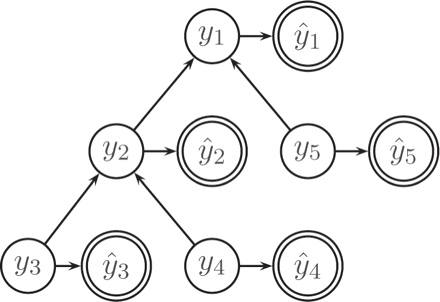
\includegraphics[width=5.5cm]{figures/net}
\caption[Example of the structure of the Bayesian network]{Simple example of the structure of the network.
Figure copied from \cite{bnet}.}
\label{fig:net}
\end{center}
\end{figure}

More formally, we want to find such consistent $y_1, ..., y_n$
(where $n$ is the number of nodes in the network)
which maximize the expression:
\[P(y_1, ..., y_n \,|\, \hat{y}_1, ..., \hat{y}_n) \propto P(\hat{y}_1, ..., \hat{y}_n\, | \, y_1, ..., y_n) \cdot P(y_1, ..., y_n). \]
Since the values $y_1, ..., y_n$ are independent, we can factor the conditional probability:
\[P(\hat{y}_1, ..., \hat{y}_n\, |\, y_1, ..., y_n) = \prod_{i=1}^n P(\hat{y_i} \,|\,y_i). \]
Note, that in where $\hat{y_i}$ is real number,
we will assume the distribution of $P(\hat{y_i}\,|\,y_i)$ to be Gaussian.

% TODO FIXME zdůvodnění proč je Gaussian
%Then the joint distribution $P(\hat{y_i}, y_i)$ would be a mixture of Gaussians
%with the mixture coefficients being the probabilities $P(y_i)$.
Provided the network structure, using the conditional independence rule,
the joint probability on $y_i$ can be factored as:
\[ P(y_1, ..., y_n) = \prod_{i=1}^n P(y_i\,|\,\{y_j : j  \,  \prec \,  i\}). \]

Now, conditional probability tables for the distributions $P(y_i\,|\,\{y_j : j  \,  \prec \,  i\})$ 
can be simply computed from \emph{training} data by counting of occurrences.
A prior count of 1 sample for each case is used to avoid the 
possibility of zero probability for some cases.
To ensure consistency of the output, however, 
we shall set:
\[ P(y_i = \top \, | \, \exists y \in \{y_j : j  \,  \prec \,  i\}, \, y = \top  ) = 1, \]
which means that a node must be positive if some more specific term is positive.
The parameters of the probabilities $P(\hat{y_i}\,|\,y_i)$ can be
calculated by taking part of the \emph{testing} data
(not used later for evaluation) to
obtain $y_i$ values and estimate the parameters of $P(\hat{y_i}\,|\,y_i)$
for example by the maximum likelihood method.
In case of a binary classifier, 
these parameters are contained within the confusion matrix divided 
by the number of tested samples.

There is one exception to the above: 
The most general function called ``molecular\_function'',
which is true for any protein
(and thus it does not even make sense to train it.)
We set the conditional probability table trivially to:
\[ P(molecular\_function = \top \,|\, anything ) = 1. \]

This assumption that the distributions of $P(\hat{y_i}\,|\,y_i)$ are Gaussian  
deserves some justification.
It is an ad-hoc assumption:
Some simple distribution is needed to for us
to be able to perform Bayesian inference
and using a continuous distribution,
already makes inference somewhat difficult.
See the Figure \ref{fig:gaussians}
for sample comparison with experimental results.
We can see that the real underlying distributions are apparently not exactly Gaussian,
but close enough to be reasonably approximated as Gaussian.
It could be examined by statistical normality tests to get more detailed view on this assumption.

\begin{figure}[h]
\begin{center}
\includegraphics[width=12cm]{figures/g}
\caption[Probability distributions of decision function values for DNA binding]{Distributions of decision function values for DNA binding protein function -- histograms of real data and estimated Gaussians;
horizontal axis shows the oriented distance from the SVM's separating hyperplane, vertical axis shows probability density.}
\label{fig:gaussians}
\end{center}
\end{figure}

Inference on this Bayesian network is done using the \emph{variational Bayes} \cite{varb} method.
Variational Bayes is an algorithm used to
obtain the approximate posterior probabilities $P(y_i \, | \, \hat{y}_1, ..., \hat{y}_n).$
It was chosen, because it can handle nodes with Gaussian distributions within the network.
Once we have the posterior probabilities, 
we can simply make the final classification by setting:
\[ y_i := P(y_i = \top \, | \, \hat{y}_1, ..., \hat{y}_n) > \frac{1}{2}, \]
for each $y_i$.

\section{Experimental settings and methodological remarks}
In this section, the experimental setting confomation and
methodology concerning the evaluation
of the experimental results are discussed.

With the filtering described in subsection \ref{ssec:proteins}
and making the dataset non-redundant as described in subsection \ref{ssec:redundancy},
we ended up with 3607 proteins.
This number is reduced to $2^{11} = 2048$ for tractability (but also aesthetical) reasons. 
This significantly more than the size of the largest data set used in the work
\cite{szabova} for DNA binding prediction,
where 138 DNA-binding and 843 non-DNA-binding (981 in total) proteins were used.

The same set is used for all studied functions.
Given this set, only functions from the Gene Ontology that have at least $2^7 = 128$
proteins associated with them (considering transitivity of $\prec$) are used.
The resulting subset of the ontology with it's structure is displayed on Figure \ref{fig:go}.
The GO identifiers and the numbers samples for each of there function is present in Table \ref{table:terms}.  
TreeLiker is then configured to run with subsampling.
That means, that RelF is ran repeatedly on a random subset of the whole data set
and in the end, it outputs the data propositionalized on the
union of features found in all iterations.
Sample size is set to $2^9=512$ and number of samples (iterations) is set to $2^3=8$.

\begin{landscape}
\begin{figure}[h]
\begin{center}
\includegraphics[width=21cm]{figures/go-basic_children}
\caption{The used subset of the Gene Ontology}
\label{fig:go}
\end{center}
\end{figure}
\end{landscape}

The following method is used to process data:
Using 8-fold cross-validation split the input proteins into folds
containing training and testing data.
RelF is ran on training data and the testing 
data are propositionalized given the features learned by RelF.
Testing data in each fold are further split into two equally sized parts,
let us call them ``test'' and ``validation'' sets.
The size of both test and validation set is thus $2048 / 8 / 2 =  128$.
Classifiers are fitted on the propositionalized training data.
The state of the art SVM classifier with Radial Basis Function (RBF)
kernel and $C = 1$ parameter is used.
Random forest and AdaBoost classifiers were also examined 
and they tend to give similar results as RBF SVM,
but the nature of their decision function is different
and would require appropriate modifications in the construction of the 
correcting Bayesian network.
The training samples are weighted in such way, that the total weights
of positive samples is equal to the total weight of negative samples.
Samples within each class have equal weights. 
(This could be refined for example by assigning lesser weight
to proteins with more unknown information.)
Subsequently the correcting Bayesian network is constructed
for each fold by taking classifiers of all functions trained
on the train set in the given fold
and the probabilities $P(\hat{y_i}\,|\,y_i)$ are estimated from the test set.
The performance of the classification both before and after the correction
is performed on the validation set.

% TODO: Výpočet jak moc vadí ne-stratifikace
This approach is not perfect. 
An noteworthy problem is that the cross-validation is not stratified,
since the folds are the same for each function.
The reason for this is is implementational, not principial:
If the folds would be stratified with respect to a given 
function, RelF could learn different features for different functions
in the same fold.
It is not possible in the TreeLiker software to 
propositionalize a relational data set given arbitrary features
(already learned on different data, in this case).
Therefore, if we kept some proteins aside from the beginning 
with the intention to use them for final evaluation,
we could not propositionalize them.
If instead we used the method described above but with stratification,
we could correctly (without information leakage) evaluate the network only with proteins
that are in the intersection of the test sets of all used functions.
It is likely that this set would be very small or even empty.

The impact of not stratifying the data set depends on the number of cross validation folds
and the ratio of samples of a given function to the data set size (see Table \ref{table:terms}).
More folds imply smaller test sets, 
which in turn increases the probability of the class representatives in test set
being disproportional to the training set.
The same follows from decreasing the ratio.
This is only globally true, but locally not monotonic, see below.

As we will see in the Results chapter, the real impact of not using stratification
in cross validation is significant.
(It even happened that a test set in a fold for a function with small number of representatives in
the original data set had zero positive examples rendering the evaluation meaningless.)
Therefore a more detailed analysis of this problem follows,
which makes for an interesting minor research problem on it's own:

Assume that the original data set has size $M$ and contains $K$
positive examples for a given function.
Now we randomly take $m$ samples to be the test set (for train set, the reasoning would be the same).
The probability that there are now $k$ positive samples 
in the test set is given by the hypergeometric probability distribution.
Now we can ask -- for a given $M, K, m$ and a constant $\alpha > 1$, what is the probability $q$ where:
\[ q = P\left(1 / \alpha \le \frac{\frac{K}{M}}{\frac{k}{m}} \le 1 \cdot \alpha \right) \,  ? \]
Simply saying: Is it probable that the ratio of positive samples in test set will be much different
from the ratio in the original set? 
Will it be at most $\alpha$-times smaller or larger?
Unfortunately, it is very complicated to work with this analytically due to the combinatorial 
nature of hypergeometric distribution.
(Read: The \texttt{FullSimplify} function in Mathematica could not work this out.)
However, it can be worked with numerically.
Figure \ref{fig:hyper} displays this piquantly non-monotonic probability for $M = 2048, m = 128, \alpha = 1.25$ and interesting 
values of $K$.
Further, the probabilities for values $\alpha \in \{1.1, 1.25, 1.5\}$ are shown in Table \ref{table:terms} 
for better insight.
We can observe, that depending on $K$, the values range from reasonable to questionable but not completely senseless.
The following Mathematica source code was used to generate the plot in Figure \ref{fig:hyper}
and it can be reused to examine this problem with general values for parameters $M,m,\alpha$:
\begin{verbatim}
M = 2048; m = 128; \[Alpha] = 1.25; minK = 128; maxK = 768;
q := Module[{K, \[Alpha]}, Function[{K, \[Alpha]}, N[
    Probability[
      1/\[Alpha] <= (K/M)/(k/m) <= \[Alpha],
      k \[Distributed] HypergeometricDistribution[m, K, M]]]]] 
ListPlot[Table[
   q[K, \[Alpha]],
   {K, minK, maxK}],
 Filling -> Axis,
 PlotStyle -> {AbsolutePointSize[1]},
 PlotRange -> {{minK, maxK}, {0, 1}},
 DataRange -> {minK, maxK},
 AxesOrigin -> {minK, 0},
 AxesLabel -> {"K", 
   "q : \[Alpha] = " <> ToString[\[Alpha]] <> ", M = " <> 
    ToString[M] <> ", m = " <> ToString[m]}]
\end{verbatim}

\begin{figure}[h]
\begin{center}
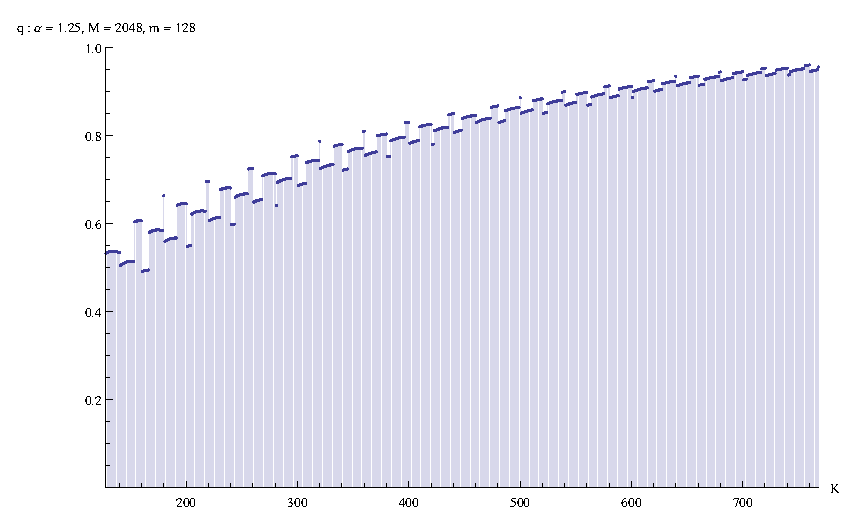
\includegraphics{figures/hyper}
\caption[Plot of probability that test set is ``stratified enough'']{Probability $q$ that test set is ``stratified enough''.
$K$ is the number of positive samples in original data set.}
\label{fig:hyper}
\end{center}
\end{figure}


% FIXME!!
\begin{table}
\begin{small}
\begin{center}
\begin{tabular}{lrrrrrl}
\textbf{GO id} & $K$ & \textbf{Ratio} & $q_{\alpha = 1.1}$ & $q_{\alpha = 1.25} $ & $q_{\alpha = 1.5}$ &  \textbf{Name} \\ \hline
GO:0003674  &  2048  &  1.00  & 1.00 & 1.00 & 1.00 &    molecular function \\ \hline
GO:0003824  &  764   &  0.37  & 0.60 & 0.95 & 1.00 &    catalytic activity \\ \hline
GO:0005488  &  1627  &  0.79  & 0.97 & 1.00 & 1.00 &    binding \\ \hline
GO:0005515  &  731   &  0.36  & 0.61 & 0.95 & 1.00 &   protein binding \\ \hline
GO:0016740  &  285   &  0.14  & 0.31 & 0.70 & 0.94 &   transferase activity \\ \hline
GO:0016787  &  290   &  0.14  & 0.31 & 0.70 & 0.93 &   hydrolase activity \\ \hline
GO:0036094  &  325   &  0.16  & 0.38 & 0.73 & 0.95 &    small molecule binding \\ \hline
GO:0043167  &  717   &  0.35  & 0.61 & 0.95 & 1.00 &    ion binding \\ \hline
GO:0097159  &  806   &  0.39  & 0.65 & 0.96 & 1.00 &    organic cyclic compound binding \\ \hline
GO:0097367  &  186   &  0.09  & 0.25 & 0.56 & 0.87 &   carbohydrate derivative binding \\ \hline
GO:1901363  &  797   &  0.39  & 0.60 & 0.97 & 1.00 &   heterocyclic compound binding \\ \hline
GO:0001882  &  156   &  0.08  & 0.27 & 0.61 & 0.81 &  nucleoside binding \\ \hline
GO:0003676  &  611   &  0.30  & 0.57 & 0.91 & 1.00 &    nucleic acid binding \\ \hline
GO:0005102  &  148   &  0.07  & 0.27 & 0.51 & 0.76 &    receptor binding \\ \hline
GO:0043168  &  256   &  0.12  & 0.32 & 0.72 & 0.93 &   anion binding \\ \hline
GO:0043169  &  520   &  0.25  & 0.47 & 0.88 & 0.99 &   cation binding \\ \hline
GO:1901265  &  279   &  0.14  & 0.40 & 0.71 & 0.94 &    nucleoside phosphate binding \\ \hline
GO:0000166  &  279   &  0.14  & 0.40 & 0.71 & 0.94 &    nucleotide binding \\ \hline
GO:0001883  &  153   &  0.07  & 0.27 & 0.51 & 0.81 &    purine nucleoside binding \\ \hline
GO:0003677  &  221   &  0.11  & 0.34 & 0.61 & 0.87 &    DNA binding \\ \hline
GO:0003723  &  199   &  0.10  & 0.24 & 0.64 & 0.86 &   RNA binding \\ \hline
GO:0032549  &  152   &  0.07  & 0.27 & 0.51 & 0.81 &    ribonucleoside binding \\ \hline
GO:0035639  &  148   &  0.07  & 0.27 & 0.51 & 0.76 &  purine ribonucleoside triphosphate binding \\ \hline
GO:0046872  &  507   &  0.25  & 0.47 & 0.86 & 0.99 &    metal ion binding \\ \hline
GO:0017076  &  154   &  0.08  & 0.27 & 0.60 & 0.81 &    purine nucleotide binding \\ \hline
GO:0032550  &  151   &  0.07  & 0.27 & 0.51 & 0.80 &   purine ribonucleoside binding \\ \hline
GO:0032553  &  157   &  0.08  & 0.27 & 0.61 & 0.82 & ribonucleotide binding \\ \hline
GO:0046914  &  220   &  0.11  & 0.34 & 0.70 & 0.87 &    transition metal ion binding \\ \hline
GO:0008270  &  185   &  0.09  & 0.25 & 0.56 & 0.87 &    zinc ion binding \\ \hline
GO:0030554  &  132   &  0.06  & 0.28 & 0.54 & 0.78 &   adenyl nucleotide binding \\ \hline
GO:0032555  &  153   &  0.07  & 0.27 & 0.51 & 0.81 &    purine ribonucleotide binding \\ \hline
GO:0032559  &  131   &  0.06  & 0.28 & 0.54 & 0.78 &   adenyl ribonucleotide binding \\ \hline
\end{tabular}
\end{center}
\end{small}
\caption{Counts of positive samples in the data set for each function.}
\label{table:terms}
\end{table}

Finally, let us remark that although cross-validation is normally used only to evaluate
the classifier performance and the final classifier is produced by training 
on the whole set, this is not done here.
The reasons are two, first the learning is already very computationally demanding
and this would make it even more and second, this work
is intended to be experimental only and the classifier will not be 
immediately applied, so it would not be useful anyway.

%*****************************************************************************
\chapter{Realization and implementation}
\label{ch:realization}
In this chapter, more technical details about the actual implementation 
of the ideas described in the previous chapter are discussed.

\section{Requirements} implementation of this work was done using combinations of Linux shell scripts
and novel software written in the Python programming language.
The scikit-learn \cite{sklearn} library was used as 
implementation of machine learning algorithms including SVM, cross validation and receiver operating characteristic evaluation.
The BayesPy (\url{http://www.bayespy.org/}) library is used for representation and inference of 
the correcting Bayesian networks.
The Matplotlib library is used to create figures presented in the results chapter \ref{ch:results}.
The dill library is necessary for data serialization done for speed and memory optimizations.
Python version $\ge$ 3.5 is required.
Finally a crucial component is the TreeLiker software,
used as RelF implementation,
which is a standalone third party product.


\section{Environment preparation} The implementation of this work can be divided into two parts that can be ran independently once some data are present:
1) Scripts that download and prepare the data.
2) Python script that performs the learning and evaluation.
We will first describe the data preparation.

First of all, the project should be configured in the \texttt{config.sh} file,
which contains mainly names of data source files and numerical parameters
such as the required data set size and so on.
There is a sample configuration file present with the name \texttt{config-sample.sh},
which should be self-explanatory.

Then the data are downloaded from the sources mentioned in section \ref{sec:data}.
Note, that the entire PDB archives (a gzipped xml file for each of the $\approx$ 110000 protein entries)
available for download using \texttt{rsync} tool add up to 42GiB to this date,
which may take a long time to download.
This can be done by running the \texttt{updatadata.sh}

Once the data are downloaded, the \texttt{blastdb.sh} script can be ran,
which filters the protein entries as described in subsection \ref{ssec:proteins}
and calculates pairwise BLAST distances. 
This is done using the offline BLAST+ software package
available at \url{ftp://ftp.ncbi.nlm.nih.gov/blast/executables/blast+/2.2.31/}
and running the \texttt{makeblastdb} and \texttt{blastp} commands. 
(See the script for details.)
The filtering results in $n > 40000$ candidate proteins.
Computing pairwise BLAST distance requires $O(n^2)$ local alignment computations.
That is a lengthy computation which took about four hours on a 3.1 GHz processor.
The results are stored and a non-redundant data set 
is generated from the candidate set using the method described in \ref{ssec:redundancy}.
The non-redundant data set can be also generated independently using the 
\texttt{dp/maximumIndependentSet.py} script.

Before the project environment is completely ready,
the script \texttt{updatadata.sh} has to be run once more before first run to prepare
serialized associations for the main program which enables it to run faster.
Then, the \texttt{run.sh} script can be ran.
(Alternatively \texttt{main.py} can be ran instead, but parameters
are not taken from \texttt{config.sh} and have to be entered in command line,
use \texttt{main.py $--$help} for details.)
There is one serious performance issue:
Depending on the protein entry size,
it can take several seconds to decompress and parse a single one.
For this reason, once parsed, the relevant data
(name, primary structure, secondary structure information and distances
between amino acid residues) is serialized and stored.
When the protein data are requested again, even in subsequent 
runs of the program, it is available quickly.

\section{Main processing} When ran the program first parses the ontology in the obo format and protein annotation file
automatically downloaded previously from Gene Ontology servers.
It clips the data set to the required maximal size and decides which
protein functions have enough positive examples in order to be studied.
For each of these functions a copy of the data set 
with the function's respective labels is
converted to the 
relational format described in \ref{ssec:relrepr} in the ``pseudo-prolog''
syntax understood by TreeLiker.
A TreeLiker batch file describing how the propositionalization
should exactly be performed including cross validation considerations
is also generated.
Then, the TreeLiker software is called as a sub-process.
That is the most computationally demanding part of the data flow.
In the described settings, it ran for approximately 23 hours for each function.
(That is almost 3 hours per cross-validation fold.)
Multiplied by 31 studied protein functions, it adds up to a month of computation time.
For this reason, the computations were run in parallel 
using the MetaCentrum/CERIT-SC computational facilities.
The intermediate results produced by TreeLiker in arff format are bzip2 compressed
and since they are text files the compression rate is very high. 
Without compression, the size of the entire working directory
would exceed the CERIT-SC (zuphux front-end machine) 104GiB disc quota.
When the propositionalization is finished,
the SVM classifiers are trained for each fold
and subsequently the correcting Bayesian networks are produced.
Then, evaluation on kept aside validation data 
and plotted ROC curve figures are saved
in the \texttt{results} folder.


%*****************************************************************************
\chapter{Experimental results}
\label{ch:results}

\begin{itemize}
 \item Způsob, průběh a výsledky testování.
 \item Srovnání s existujícími řešeními, pokud jsou známy.
\end{itemize} 


%*****************************************************************************
\chapter{Conclusion}

\begin{itemize}
\item Zhodnocení splnění cílů DP/BP a  vlastního přínosu práce (při formulaci je třeba vzít v potaz zadání práce).
\item Diskuse dalšího možného pokračování práce.\end{itemize}   note={\url{http://geneontology.org/}},


%*****************************************************************************
% Seznam literatury je v samostatnem souboru reference.bib. Ten
% upravte dle vlastnich potreb, potom zpracujte (a do textu
% zapracujte) pomoci prikazu bibtex a nasledne pdflatex (nebo
% latex). Druhy z nich alespon 2x, aby se poresily odkazy.

%\bibliographystyle{abbrv}
\bibliographystyle{plain}
%\bibliographystyle{alpha}
%\bibliographystyle{psc}
{
%JZ: 11.12.2008 Kdo chce mit v techto ukazkovych odkazech take odkaz na CSTeX:
\def\CS{$\cal C\kern-0.1667em\lower.5ex\hbox{$\cal S$}\kern-0.075em $}
\bibliography{reference}
}

% M. Dušek radi:
%\bibliographystyle{alpha}
% kdy citace ma tvar [AutorRok] (napriklad [Cook97]). Sice to asi neni  podle ceske normy (BTW BibTeX stejne neodpovida ceske norme), ale je to nejprehlednejsi.
% 3.5.2009 JZ polemizuje: BibTeX neobvinujte, napiste a poskytnete nam styl (.bst) splnujici citacni normu CSN/ISO.

%*****************************************************************************
%*****************************************************************************
%*****************************************************************************
\chapter{Pokyny a návody k formátování textu práce}
\textbf{\large Tato příloha samozřejmě nebude součástí vaší práce. Slouží pouze jako příklad formátování textu.}

Používat se dají všechny příkazy systému \LaTeX. Existuje velké množství volně přístupné dokumentace, tutoriálů, příruček a dalších materiálů v elektronické podobě. Výchozím bodem, kromě Googlu, může být stránka CSTUG (Czech Tech Users Group) \cite{CSTUG}. Tam najdete odkazy na další materiály.  Vetšinou dostačující a přehledně organizovanou elektronikou dokumentaci najdete například na \cite{latexdocweb} nebo \cite{latexwiki}.

Existují i různé nadstavby nad systémy \TeX{} a \LaTeX, které výrazně usnadní psaní textu zejména začátečníkům. Velmi rozšířený v Linuxovém prostředí je systém Kile.


\section{Vkládání obrázků}
Obrázky se umísťují do plovoucího prostředí \verb|figure|. Každý obrázek by měl obsahovat \textbf{název} (\verb|\caption|) a \textbf{návěští} (\verb|\label|). Použití příkazu pro vložení obrázku \\\verb|\includegraphics| je podmíněno aktivací (načtením) balíku graphicx příkazem\\ \verb|\usepackage{graphicx}|.

Budete-li zdrojový text zpracovávat pomocí programu \verb|pdflatex|, očekávají se obrázky s příponou \verb|*.pdf|\footnote{pdflatex umí také formáty PNG a JPG.}, použijete-li k formátování \verb|latex|, očekávají se obrázky s příponou \verb|*.eps|.\footnote{Vzájemnou konverzi mezi snad všemi typy obrazku včetně změn vekostí a dalších vymožeností vám může zajistit balík ImageMagic  (http://www.imagemagick.org/script/index.php). Je dostupný pod Linuxem, Mac OS i MS Windows. Důležité jsou zejména příkazy convert a identify.}

\begin{figure}[ht]
\begin{center}

\includegraphics[width=5cm]{figures/LogoCVUT}
\caption{Popiska obrázku}
\label{fig:logo}
\end{center}
\end{figure}

Příklad vložení obrázku:
\begin{verbatim}
\begin{figure}[h]
\begin{center}

\includegraphics[width=5cm]{figures/LogoCVUT}
\caption{Popiska obrazku}
\label{fig:logo}
\end{center}
\end{figure}
\end{verbatim}

\section{Kreslení obrázků}
Zřejmě každý z vás má nějaký oblíbený nástroj pro tvorbu obrázků. Jde jen o to, abyste dokázali obrázek uložit v požadovaném formátu nebo jej do něj konvertovat (viz předchozí kapitola). Je zřejmě vhodné kreslit obrázky vektorově. Celkem oblíbený, na ovládání celkem jednoduchý a přitom dostatečně mocný je například program Inkscape.

Zde stojí za to upozornit na kreslící programe Ipe \cite{ipe}, který dokáže do obrázku vkládat komentáře přímo v latexovském formátu (vzroce, stejné fonty atd.). Podobné věci umí na Linuxové platformě nástroj Xfig. 

Za pozornost ještě stojí schopnost editoru Ipe importovat obrázek (jpg nebo bitmap) a krelit do něj latexovské popisky a komentáře. Výsledek pak umí exportovat přímo do pdf.

\section{Tabulky}
Existuje více způsobů, jak sázet tabulky. Například je možno použít prostředí \verb|table|, které je velmi podobné prostředí \verb|figure|. 

\begin{table}
\begin{center}
\begin{tabular}{|c|l|l|}
\hline
\textbf{DTD} & \textbf{construction} & \textbf{elimination} \\
\hline
$\mid$ & \verb+in1|A|B a:sum A B+ & \verb+case([_:A]a)([_:B]a)ab:A+\\
&\verb+in1|A|B b:sum A B+ & \verb+case([_:A]b)([_:B]b)ba:B+\\
\hline
$+$&\verb+do_reg:A -> reg A+&\verb+undo_reg:reg A -> A+\\
\hline
$*,?$& the same like $\mid$ and $+$ & the same like $\mid$ and $+$\\
& with \verb+emtpy_el:empty+ & with \verb+emtpy_el:empty+\\
\hline
R(a,b) & \verb+make_R:A->B->R+ & \verb+a: R -> A+\\
 & & \verb+b: R -> B+\\
\hline
\end{tabular}
\end{center}
\caption{Ukázka tabulky}
\label{tab:tab1}
\end{table}

Zdrojový text tabulky \ref{tab:tab1} vypadá takto:
\begin{verbatim}
\begin{table}
\begin{center}
\begin{tabular}{|c|l|l|}
\hline
\textbf{DTD} & \textbf{construction} & \textbf{elimination} \\
\hline
$\mid$ & \verb+in1|A|B a:sum A B+ & \verb+case([_:A]a)([_:B]a)ab:A+\\
&\verb+in1|A|B b:sum A B+ & \verb+case([_:A]b)([_:B]b)ba:B+\\
\hline
$+$&\verb+do_reg:A -> reg A+&\verb+undo_reg:reg A -> A+\\
\hline
$*,?$& the same like $\mid$ and $+$ & the same like $\mid$ and $+$\\
& with \verb+emtpy_el:empty+ & with \verb+emtpy_el:empty+\\
\hline
R(a,b) & \verb+make_R:A->B->R+ & \verb+a: R -> A+\\
 & & \verb+b: R -> B+\\
\hline
\end{tabular}
\end{center}
\caption{Ukázka tabulky}
\label{tab:tab1}
\end{table}
\begin{table}
\end{verbatim}

\section{Odkazy v textu}
\subsection{Odkazy na literaturu}
Jsou realizovány příkazem \verb|\cite{odkaz}|. 

Seznam literatury je dobré zapsat do samostatného souboru a ten pak zpracovat programem bibtex (viz soubor \verb|reference.bib|). Zdrojový soubor pro \verb|bibtex| vypadá například takto:
\begin{verbatim}
@Article{Chen01,
  author  = "Yong-Sheng Chen and Yi-Ping Hung and Chiou-Shann Fuh",
  title   = "Fast Block Matching Algorithm Based on 
             the Winner-Update Strategy",
  journal = "IEEE Transactions On Image Processing",
  pages   = "1212--1222",
  volume  =  10,
  number  =   8,
  year    = 2001,
}

@Misc{latexdocweb,
  author  = "",
  title   = "{\LaTeX} --- online manuál",
  note    = "\verb|http://www.cstug.cz/latex/lm/frames.html|",
  year    = "",
}
...
\end{verbatim}

%11.12.2008, 3.5.2009
\textbf{Pozor:} Sazba názvů odkazů je dána Bib\TeX{} stylem\\ (\verb|\bibliographystyle{abbrv}|). 
%Budete-li používat české prostředí (\verb|\usepackage[czech]{babel}|), 
Bib\TeX{} tedy obvykle vysází velké pouze počáteční písmeno z názvu zdroje, 
ostatní písmena zůstanou malá bez ohledu na to, jak je napíšete. 
Přesněji řečeno, styl může zvolit pro každý typ publikace jiné konverze. 
Pro časopisecké články třeba výše uvedené, jiné pro monografie (u nich často bývá 
naopak velikost písmen zachována).

Pokud chcete Bib\TeX u napovědět, která písmena nechat bez konverzí 
(viz \texttt{title = "\{$\backslash$LaTeX\} -{}-{}- online manuál"} 
v~předchozím příkladu), je nutné příslušné písmeno (zde celé makro) uzavřít 
do složených závorek. Pro přehlednost je proto vhodné celé parametry 
uzavírat do uvozovek (\texttt{author = "\dots"}), nikoliv do složených závorek.

Odkazy na literaturu ve zdrojovém textu se pak zapisují:
\begin{verbatim}
Podívejte se na \cite{Chen01}, 
další detaily najdete na \cite{latexdocweb}
\end{verbatim}

Vazbu mezi soubory \verb|*.tex| a \verb|*.bib| zajistíte příkazem 
\verb|\bibliography{}| v souboru \verb|*.tex|.  V našem případě tedy zdrojový 
dokument \verb|thesis.tex| obsahuje příkaz\\
\verb|\bibliography{reference}|.

Zpracování zdrojového textu s odkazy se provede postupným voláním programů\\
\verb|pdflatex <soubor>| (případně \verb|latex <soubor>|), \verb|bibtex <soubor>| 
a opět\\ \verb|pdflatex <soubor>|.\footnote{První volání \texttt{pdflatex} 
vytvoří soubor s~koncovkou \texttt{*.aux}, který je vstupem pro program 
\texttt{bibtex}, pak je potřeba znovu zavolat program \texttt{pdflatex} 
(\texttt{latex}), který tentokrát zpracuje soubory s příponami \texttt{.aux} a 
\texttt{.tex}. 
Informaci o případných nevyřešených odkazech (cross-reference) vidíte přímo při 
zpracovávání zdrojového souboru příkazem \texttt{pdflatex}. Program \texttt{pdflatex} 
(\texttt{latex}) lze volat vícekrát, pokud stále vidíte nevyřešené závislosti.}


Níže uvedený příklad je převzat z dříve existujících pokynů studentům, kteří 
dělají svou diplomovou nebo bakalářskou práci v~Grafické skupině.\footnote{Několikrát 
jsem byl upozorněn, že web s těmito pokyny byl zrušen, proto jej zde přímo necituji. 
Nicméně příklad sám o sobě dokumentuje obecně přijímaný konsensus ohledně citací 
v~bakalářských a diplomových pracích na KP.} Zde se praví:
\begin{small}
\begin{verbatim}
...
j) Seznam literatury a dalších použitých pramenů, odkazy na WWW stránky, ...
 Pozor na to, že na veškeré uvedené prameny se musíte v textu práce 
 odkazovat -- [1]. 
Pramen, na který neodkazujete, vypadá, že jste ho vlastně nepotřebovali 
a je uveden jen do počtu. Příklad citace knihy [1], článku v časopise [2], 
stati ve sborníku [3] a html odkazu [4]: 
[1] J. Žára, B. Beneš;, and P. Felkel. 
     Moderní počítačová grafika. Computer Press s.r.o, Brno, 1 edition, 1998. 
     (in Czech). 
[2] P. Slavík. Grammars and Rewriting Systems as Models for Graphical User 
     Interfaces. Cognitive Systems, 4(4--3):381--399, 1997. 
[3] M. Haindl, Š. Kment, and P. Slavík. Virtual Information Systems. 
     In WSCG'2000 -- Short communication papers, pages 22--27, Pilsen, 2000. 
     University of West Bohemia. 
[4] Knihovna grafické skupiny katedry počítačů: 
     http://www.cgg.cvut.cz/Bib/library/ 
\end{verbatim}
\end{small}
\ldots{} abychom výše citované odkazy skutečně našli v (automaticky generovaném) seznamu literatury tohoto textu, musíme je nyní alespoň jednou citovat: Kniha \cite{kniha}, článek v~časopisu \cite{clanek}, příspěvek na konferenci \cite{sbornik}, www odkaz \cite{www}.

\subsection{Odkazy na obrázky, tabulky a kapitoly}
\begin{itemize}
\item Označení místa v textu, na které chcete později čtenáře práce odkázat, se provede příkazem \verb|\label{navesti}|. Lze použít v prostředích \verb|figure| a  \verb|table|, ale též za názvem kapitoly nebo podkapitoly.
\item Na návěští se odkážeme příkazem \verb|\ref{navesti}| nebo \verb|\pageref{navesti}|.
\end{itemize}

\section{Rovnice, centrovaná, číslovaná matematika}
Jednoduchý matematický výraz zapsaný přímo do textu se vysází pomocí prostředí \verb|math|, resp. zkrácený zápis pomocí uzavření textu rovnice mezi znaky \verb|$|.

Kód \verb|$ S = \pi * r^2 $| bude vysázen takto: $ S = \pi * r^2 $.

Pokud chcete nečíslované rovnice, ale umístěné centrovaně na samostatné řádky, pak lze použít prostředí \verb|displaymath|, resp. zkrácený zápis pomocí uzavření textu rovnice mezi znaky \verb|$$|. Zdrojový kód: 
\begin{verb}
|$$ S = \pi * r^2 $$|
\end{verb}
bude pak vysázen takto:
$$ S = \pi * r^2 $$

Chcete-li mít rovnice číslované, je třeba použít prostředí \verb|eqation|. Kód:
\begin{verbatim}
\begin{equation}
  S = \pi * r^2
\end{equation}

\begin{equation}
  V = \pi * r^3
\end{equation}
\end{verbatim}
je potom vysázen takto:
\begin{equation}
  S = \pi * r^2
\end{equation}

\begin{equation}
  V = \pi * r^3
\end{equation}

\section{Kódy programu}
Chceme-li vysázet například část zdrojového kódu programu (bez formátování), hodí se prostředí \verb|verbatim|: 
\begin{verbatim}
         (* nickname2 *)
Lego> Refine in1
             (do_reg (nickname1 h));
Refine by  in1 (do_reg (nickname1 h))
   ?4 : pcdata
   ?5 : pcdata
          (* surname2 *)
Lego> Refine surname1 h;
Refine by  surname1 h
   ?5 : pcdata
          (* email2 *)
Lego> Refine undo_reg (email1 h);
Refine by  undo_reg (email1 h)
*** QED ***
\end{verbatim}

\section{Další poznámky}
\subsection{České uvozovky}
V souboru \verb|k336_thesis_macros.tex| je příkaz \verb|\uv{}| pro sázení českých uvozovek. \uv{Text uzavřený do českých uvozovek.}

% JZ: 3.5.2009 \chapter z book zajistí automaticky
%\subsection{Začátky kapitol na liché stránky}
%Ve výsledném textu je dobré, když každá kapitola začíná na liché stránce. Tedy použijte:
%\begin{verbatim}
%  \cleardoublepage\include{1_uvod}
%  \cleardoublepage\include{2_teorie}
%   atd.\ldots{}
%\end{verbatim}

%*****************************************************************************
\chapter{Seznam použitých zkratek}

\begin{description}
\item[2D] Two-Dimensional
\item[ABN] Abstract Boolean Networks
\item[ASIC] Application-Specific Integrated Circuit
\end{description}
\vdots

%*****************************************************************************
\chapter{UML diagramy}
\textbf{\large Tato příloha není povinná a zřejmě se neobjeví v každé práci. Máte-li ale větší množství podobných diagramů popisujících systém, není nutné všechny umísťovat do hlavního textu, zvláště pokud by to snižovalo jeho čitelnost.}

%*****************************************************************************
\chapter{Instalační a uživatelská příručka}
\textbf{\large Tato příloha velmi žádoucí zejména u softwarových implementačních prací.}

%*****************************************************************************
\chapter{Obsah přiloženého CD}
\textbf{\large Tato příloha je povinná pro každou práci. Každá práce musí totiž obsahovat přiložené CD. Viz dále.}

Může vypadat například takto. Váš seznam samozřejmě bude odpovídat typu vaší práce. (viz \cite{infodp}):

\begin{figure}[h]
\begin{center}
\includegraphics[width=14cm]{figures/seznamcd}
\caption{Seznam přiloženého CD --- příklad}
\label{fig:seznamcd}
\end{center}
\end{figure}

Na GNU/Linuxu si strukturu přiloženého CD můžete snadno vyrobit příkazem:\\ 
\verb|$ tree . >tree.txt|\\
Ve vzniklém souboru pak stačí pouze doplnit komentáře.

Z \textbf{README.TXT} (případne index.html apod.)  musí být rovněž zřejmé, jak programy instalovat, spouštět a jaké požadavky mají tyto programy na hardware.

Adresář \textbf{text}  musí obsahovat soubor s vlastním textem práce v PDF nebo PS formátu, který bude později použit pro prezentaci diplomové práce na WWW.

\end{document}
